\documentclass[a4paper,twoside]{article}

%
%  P R E A M B L E
%

\usepackage{graphicx}
\usepackage{natbib}
\usepackage{xspace}
\usepackage{makeidx}
\usepackage{dcolumn}
\usepackage{slashbox}

\newcolumntype{d}[1]{D{.}{.}{#1}}


\makeindex

\newcommand{\cobalt}{Cobalt\xspace}
\newcommand{\bgp}{BG/P\xspace}
\newcommand{\cep}{CEP-2\xspace}

\newcommand{\dm}{\mathrm{DM}}

\newcommand{\fftwforward}{\texttt{FFTW\_FORWARD}\xspace}
\newcommand{\fftwbackward}{\texttt{FFTW\_BACKWARD}\xspace}



%
%  D O C U M E N T
%

\title{Cobalt beam former algorithmic design version 0.2}
\author{M.A. Brentjens}



\begin{document}

\maketitle

\tableofcontents

\pagebreak


%
% Introduction
%

\section{Introduction}

\cobalt is LOFAR's new digital back end, succeeding the \bgp at
2013-12-31 at the latest \citep{CobaltRequirements2013}. It will
consist of several Linux servers equipped with NVIDIA Graphical
Processing Units (GPUs), interconnected by an infiniband network.  The
GPUs will do most of the number crunching, while the servers
themselves are responsible for data I/O and higher level logic.

Besides cross-correlating station data streams to produce
interferometric visibilities, \cobalt will be combining data
streams from multiple stations by coherently or incoherently adding
them. This is done by the beam former pipeline.

This memo presents a mathematical description of the \cobalt beam
former pipeline, including an analysis of delay compensation%,
% data
%flagging and excision at various stages of the processing,
and a proposal for a coherent dedispersion algorithm that properly takes
into account all relevant preceding and succeeding time frames.




%
%  High level design
%

\section{High level design}

\begin{figure}
\begin{center}
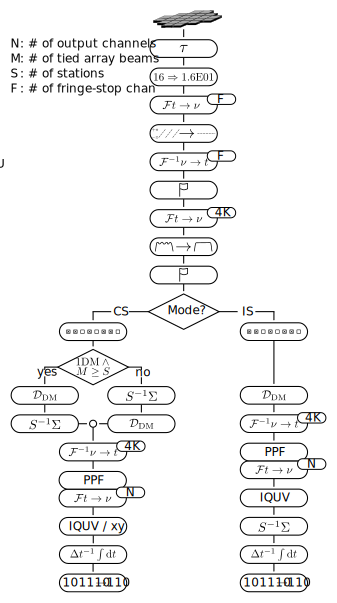
\includegraphics[height=0.9\textheight]{cobalt-beam-former-pipeline-bw.pdf}
\end{center}
\caption{High level flow diagram of the \cobalt tied array beam former
  pipeline for a single sub band.}
\label{fig:pipeline-overview}
\end{figure}


\cobalt supports coherent and incoherent addition of station data. A
fly's eye mode, in which all stations may point in \emph{different}
directions, is implemented through multiple parallel observations. All
modes allow optional online coherent dedispersion. If time permits,
online flagging of broad-band pulsed RFI and narrow band RFI will be
implemented on the station streams, and bit-reduction will be
implemented just before writing the data to storage.

Figure~\ref{fig:pipeline-overview} gives an overview of the successive
operations performed on a single sub band's data by \cobalt's beam
former pipeline. 

\subsection{Per station}

The first step is full sample delay compensation of the incoming
station data at a resolution of 5.12 or 6.4~$\mu$s for the 200 and
160~MHz clocks, respectively. The delay that is compensated for is the
sum of the geometrical delay, known clock delay, and normalization
delays per polarization and antenna set at the stations due to station
calibration. In other words, the total delay from the moment the wave
front hits the antenna set's phase centre until time stamping at the
RSP boards just before the data are sent to Groningen.

This is followed by conversion of the samples from integers to
floats. Fringe stopping is done by taking an $F$-point FFT,
multiplying by a phase slope across the band, and an inverse $F$-point
FFT. The upper limit to the transform length $F$ is determined by the
maximum allowable time between sub-sample delay compensation
corrections. See Sect.~\ref{sec:delay-compensation} for details.

At this stage, each sample again has the full band width of the sub
band. The high time resolution allows for sensitive flagging of broad
band, impulsive interference. The data stream is subsequently Fourier
transformed to the frequency domain. To guarantee sufficient
parallelism, this must be at least a 4096 point transform, but
coherent dedispersion may require even more micro-channels. At this
stage, the station's poly phase filter's band pass is compensated, and
we allow for additional flagging of narrow-band interference.

All steps until now have been performed on the data streams from
individual stations. What happens next depends on which data products
are required. Each data product is a combination of data from one or
more stations. For each data product, one must therefore make a
selection of stations required to compute it.


\subsection{Coherent Stokes}

The coherent stokes mode performs coherent averaging of one or more
stations. If coherent dedispersion is required, this can be done
either before, or after the averaging of the complex voltages. If the
number of tied array beams $M$ is larger than the number of stations
$S$, and every tied array beam has the same dispersion measure, it
will be done before averaging, otherwise afterwards. This
approach maximizes the amount of memory available to buffer data for
compensating large dispersion measures at low frequencies.

There is much more memory available at the CPUs than at the GPUs, so
preferably, coherent dedispersion is done in CPU
memory. Unfortunately, it is not yet clear if the band width between
GPU and CPU memory is large enough to accommodate the data rate.

After coherent dedispersion and averaging over the stations, the data
are Fourier transformed back to the maximum time resolution. In
Fig.~\ref{fig:pipeline-overview} this is indicated by a $4\mathrm{K}$
inverse Fourier transform. Evidently, this transform must have the
same length as the Fourier transform before correction of the
station's poly phase filter band pass. The data are transformed to the
final frequency resolution using a combination of a 16-tap poly phase
filter (PPF) and a Fourier transform to guarantee excellent channel
separation.

If the user required Stokes parameters, they are computed at this
stage. For complex voltages in $x$ and $y$, the Stokes conversion step
is skipped. Note that the Stokes parameters are not Stokes parameters
in the IAU definition and celestial reference frame, but rather just
\begin{eqnarray}
I &=& x x^* + y y* \\
Q &=& x x^* - y y^* \\
U &=& x y^* + y x^* \\
V &=& \mathrm{i}\left(x y^* - y x^* \right)
\end{eqnarray}
These quantities can be converted to true astronomical Stokes
parameters by applying the appropriate Mueller matrix of the element
beam during post processing.

The final time resolution of the data can optionally be reduced by
averaging spectra in time before writing them to the storage
cluster. The pulsar group also requests an optional bit reduction step
to reduce the data rate by a factor up to 4. This will only be
implemented if time permits.


\subsection{Incoherent Stokes}

The incoherent Stokes mode uses the same processing steps as the
coherent Stokes mode, but in a different order. For incoherent
averaging, the Stokes conversion is always required, and must be done
\emph{before} averaging the station streams. A direct consequence in
this design is that dedispersion of incoherent stokes data will
only be implemented \emph{before} averaging the station streams.


\subsection{Fly's eye}

Fly's eye observations, in which all stations may be pointing in
different, independent directions, will be implemented as parallel
observations. A limited fly's eye mode, with all stations pointing in
the same direction, but recording data for each station individually,
can be implemented as a single observation with one tied array beam
per station and a different station selected for each tied array beam.




\section{Fourier transforms}

For developing a constant flux scale at the output of Cobalt, it is
important that all Fourier transform pairs are normalized. \cobalt
uses the FFTW library to implement the Fourier transforms. The time
domain to frequency transforms are using \fftwforward, which
computes
\begin{equation}
y_i = \sum_{j=0}^{n-1}x_j\mathrm{e}^{-2\pi\mathrm{i} i j / n},
\end{equation}
where $\mathrm{i} = \sqrt{-1}$. The frequency-to-time domain
transforms use \fftwbackward:
\begin{equation}
y_i = \sum_{j=0}^{n-1}x_j\mathrm{e}^{+2\pi\mathrm{i} i j / n}.
\end{equation}

From the FFTW manual:
\begin{quotation}

FFTW computes an unnormalized transform, that is, the equation
$\mathcal{F}^{-1}(\mathcal{F}(\vec{x})) = n \vec{x}$ holds. In other
words, applying the forward and then the backward transform will
multiply the input by $n$.

An \fftwforward transform corresponds to a sign of $-1$ in the exponent
of the DFT. Note also that we use the standard "in-order" output
ordering~--~the $k$-th output corresponds to the frequency $k/n$ (or $k/t$,
where $t$ is your total sampling period). For those who like to think in
terms of positive and negative frequencies, this means that the
positive frequencies are stored in the first half of the output and
the negative frequencies are stored in backwards order in the second
half of the output. (The frequency $-k/n$ is the same as the frequency
$(n-k)/n$.)
\end{quotation}

To make the amplitude of an astrophysical signal independent of the
number of channels that is used, the output of the
time-to-frequency transforms (\fftwforward) must be divided by
the number of points in that transform. The transforms back to the
time domain (\fftwbackward) may then \emph{not} be normalized.





%
% Delay compensation
%

\section{Delay compensation}
\label{sec:delay-compensation}



The path length difference between radiation from a source arriving at
the centre of LOFAR (CS002LBA), and at a distant station, changes as a
function of time due to the earth's rotation. The rate of change is
largest for stations exactly east or west of the centre and with the
source at transit mid-way between the centre and that station.

In this configuration, the maximum rate of change in the path length
towards a source at declination $\delta$ is
\begin{equation}
\dot{s} = \omega_\mathrm{e} d \cos \delta\ \mathrm{m}\ \mathrm{s}^{-1},
\end{equation}
where $\omega_\mathrm{e} = 7.29211585 \cdot 10^{-5}$~rad~s$^{-1}$ is the
sidereal angular velocity of the earth, and $d$ is the distance
between the station and LOFAR's core in m. The same equation can be
written in units of time:
\begin{equation}
\dot{\tau} = \frac{\omega_\mathrm{e}}{c} d \cos \delta\ \mathrm{s}\ \mathrm{s}^{-1},
\end{equation}
where $c$ is the speed of light in vacuo, or in phase:
\begin{equation}
\dot{\phi} = \frac{2\pi\nu\omega_\mathrm{e}}{c} d \cos \delta\ \mathrm{rad}\ \mathrm{s}^{-1}.
\end{equation}

Fringe stopping of the residual delay is done at an interval
$t_\mathrm{u}$. If $t_\mathrm{u}$ is too large, the signal will
decorrelate by a fraction
\begin{equation}
f_\mathrm{d} = 1 - \frac{\sin \frac{1}{2}\Delta\phi}{\frac{1}{2}\Delta\phi},
\end{equation}
where $\Delta\phi$ is the phase change over the interval
$t_\mathrm{u}$. For a dynamic range of order 1\,000\,000:1, given a
point spread function with side lobes at the $10^{-3}$ level, one
requires the visibility amplitudes to be good to about 1 part in a
1\,000. When $\Delta\phi \ll 1$,
\begin{equation}
f_\mathrm{d} \approx \frac{\Delta\phi^2}{24},
\label{eq:decorrelation-fraction}
\end{equation}
hence
\begin{equation}
\Delta\phi \approx \sqrt{24 f_\mathrm{d}}.
\end{equation}
Filling in $f_\mathrm{d} \le 10^{-3}$ yields $\Delta\phi \le
0.155$~rad, or $\Delta\phi \le 8.9^\circ$. The interval $t_\mathrm{u}$
is then given by
\begin{equation}
t_\mathrm{u} = \frac{\Delta \phi}{\dot{\phi}}.
\end{equation}
These update intervals, along with the corresponding maximum FFT lengths for
the 200~MHz clock, are listed in
Tab.~\ref{tab:delay-update-intervals}. The FFT lengths are calculated
as follows:
\begin{equation}
n_\mathrm{FFT} \le t_\mathrm{u}\frac{\nu_\mathrm{clk}}{1024},
\label{eq:fft-length}
\end{equation}
where $\nu_\mathrm{clk}$ is the clock frequency at the stations:
either 200 or 160~MHz.



\begin{table}
\caption{Maximum delay rates for core, remote, and international
  stations. Includes phase rates at 80, 180, and
  250~MHz.}
\begin{center}
\begin{tabular}{l|lllll}
\hline
\hline
Distance & $\dot{s}$    & $\dot{\tau}$   & $\dot{\phi}_{80}$ & $\dot{\phi}_{180}$ & $\dot{\phi}_{250}$ \\
 (km)    &  (m s$^{-1}$) &  (ns s$^{-1}$) & (rad s$^{-1}$)    & (rad s$^{-1}$)     & (rad s$^{-1}$)     \\
\hline
3        & 0.219        & 0.730          & 0.367            & 0.825             & 1.15              \\
100      & 7.29         & 24.3           & 12.2             & 27.5              & 38.2              \\
1500     & 109          & 365            & 183.4            & 412               & 573               \\
\hline
\hline
\end{tabular}
\end{center}
\end{table}


\begin{table}
\caption{Maximum update interval and FFT length for sub-sample delay
  compensation for core, remote, and international stations 80, 180,
  and 250~MHz. $t_\mathrm{u}$ is the maximum allowed interval between
  successive fringe corrections. $n_\mathrm{FFT}$ is computed for the
  200~MHz clock.}
\label{tab:delay-update-intervals}
\begin{center}
\begin{tabular}{l|ll|ll|ll}
\hline
\hline
Distance &  $t_\mathrm{u,80}$ & $n_\mathrm{FFT}$ & $t_\mathrm{u,180}$ & $n_\mathrm{FFT}$& $t_\mathrm{u,250}$ & $n_\mathrm{FFT}$\\
 (km)    &  (ms)             &                 & (ms)             &                & (ms)              & \\
\hline
3        &  422              & 82421           & 188              &  36718         & 135               & 26367\\
100      &   12.7            &  2480           &  5.64            &   1101         &   4.05            &   791\\
1500     &     0.845         &   165           &  0.376           &     73         &   0.271           &    53\\
\hline
\hline
\end{tabular}
\end{center}
\end{table}





Because the fringe correction is done by applying a per-channel phase
rotation, only the centre of each channel is fully corrected. Within a
channel, there remains a phase slope that goes back and forth at the
same interval, and with the same slope as a function of frequency as
the one that is being corrected for the sub band as a whole. The
amplitude of this phase wiggle at the edge of a channel is $\Delta\phi
= \frac{2\pi}{n_\mathrm{ch}}$, where $n_\mathrm{ch}$ is the number of
channels in a sub band. This leads to a small amount of decorrelation,
increasing towards the edges of the channels used for fringe
stopping. The average decorrelation within a channel is thus given by
the integral of Eq.~(\ref{eq:decorrelation-fraction}) over the channel
width:
\begin{equation}
f_\mathrm{d,ch} = 2\int_0^{2\pi/n_\mathrm{ch}} \frac{\phi^2}{24}\ \mathrm{d}\phi.
\end{equation}

Solving for $n_\mathrm{ch}$:
\begin{equation}
n_\mathrm{ch} = \pi\sqrt[3]{\frac{2}{9f_\mathrm{d,ch}}}.
\label{eq:min-number-of-channels}
\end{equation}
Filling in $f_\mathrm{d} \le 10^{-3}$ yields $n_\mathrm{ch} \ge
19$. Of course, because we are in the complex domain, $n_\mathrm{FFT}$
from Eq.~(\ref{eq:fft-length}) is equal to $n_\mathrm{ch}$ in
Eq.~(\ref{eq:min-number-of-channels}). The optimum FFT length in terms
of delay compensation accuracy and decorrelation, seems therefore given
by the maximum of 32 and the first power of two below $n_\mathrm{FFT}$
as given in Eq.~(\ref{eq:fft-length}).


Path length differences up to 1500~km must be computed with errors of
at most about 6 cm, but preferably much smaller (mm). This implies one
needs at least 7 significant digits in the computation of the path
length difference, requiring double precision numbers in the
calculation thereof. Once this delay is divided into an integer number
of time samples and a fractional sample delay, application of the sub
sample delay (fringe stopping) can easily be done in single precision.



%
% Int to float conversion
%

\section{Int to float conversion}

Here, the constant scaling factor of 16 between 8-bit and 16-bit mode
should be applied. That is, 8-bit data must be multiplied by a factor
16 when they are converted to floats. 16-bit data can be left as-is.
 


%
% Online flagging
%

\section{Online flagging}
\label{sec:online-flagging}


Because all streams of station data are added in real time, beam
formed observations are very sensitive to radio frequency interference
(RFI) at the stations. One misbehaving station, electric fence, or
thunderstorm, can ruin an entire observation. This is why the LOFAR
pulsar group requests the ability to excise suspicious data
at the station level, before the station data streams are combined.


Question: Replace with zeroes?

Question: Propagate flag mask?

Question: Propagate flag count?






%
% Station PPF correction
%

\section{Station PPF correction}
\label{sec:station-PPF-correction}

The station poly phase filter correction will be computed in the same
way as is done on the \bgp. The main difference in the application is
that that is happening at (much) higher frequency resolution here.

%
% Coherent dedispersion
%

\section{Coherent dedispersion}
\label{sec:coherent-dedispersion}

The interstellar medium (ISM) disperses cosmic radio signals propagating
through it. Signals arrive later at lower frequencies. The delay
\begin{equation}
t     =  \mathcal{D} \left(\frac{\dm}{\nu^2}\right),
\end{equation}
where the dispersion measure
\begin{equation}
\dm    =  \int_0^d n_\mathrm{e}(s)\ \mathrm{d}s\ \mathrm{pc}\ \mathrm{cm}^{-3},
\end{equation}
and the dispersion constant
\begin{equation}
\mathcal{D}  =   \frac{k_\mathrm{e}e^2}{2 \pi m_\mathrm{e} c} \approx
4148.808 \pm 0.003 \ \mathrm{MHz}^2\ \mathrm{pc}^{-1}\ \mathrm{cm}^{3}\ \mathrm{s}.
\end{equation}


Because the delay $t$ is proportional to the square of the wave
length, absolute delays of minutes to hours are possible in the lower
end of the LOFAR frequency range. For example, the Lorimer burst
($\mathrm{DM} \approx 375\ \mathrm{pc}\ \mathrm{cm}^{-3}$) would be
delayed by almost half an hour at 30~MHz.

Fortunately, only the differential delay between the top and bottom of
a sub band determines the smearing within a sub band, not the absolute
delay. For the same burst at 30~MHz, the differential delay across a
sub band is ``only'' 22 seconds. Table~\ref{tab:differential-delays}
lists differential delays for a number of (very) high dispersion
measures at several representative LOFAR frequencies.

\begin{table}
\caption{Differential dispersion delays in seconds across a sub
  band of 195~kHz (200~MHz clock).}
\label{tab:differential-delays}
\begin{center}
\begin{tabular}{r|lllll}
\hline
\hline
$\nu$ (MHz)& 30 & 50  & 110  & 150  & 210 \\
DM (pc cm$^{-3}$) \\
\hline
100        &  6  & 1.3 & 0.12 & 0.05 & 0.017\\
500        &  30 & 6.5 & 0.61 & 0.24 & 0.087\\
2500       & 150 & 32  & 3.04 & 1.20 & 0.437\\
\hline
\hline
\end{tabular}
\end{center}
\end{table}

To correct for dispersion, one needs to apply a frequency dependent
delay to the data. In the current \bgp implementation, this is done by
computing $\tau_k$, the delay between channel $k$ and the central
frequency of the sub band, converting this delay to a complex phase
factor
\begin{equation}
\mathrm{e}^{+2\pi\mathrm{i}(\nu_k-\nu_\mathrm{c})\tau_k},
\label{eq:chirp-phase}
\end{equation}
with
\begin{equation}
\tau_k =  \mathcal{D} \times \dm \times\left(\frac{1}{\nu_k^2}  -
\frac{1}{\nu_\mathrm{c}^2}\right),
\label{eq:channel-dispersion-delay}
\end{equation}
where $\nu_\mathrm{c}$ is the frequency of the sub band's central
channel, and $\nu_k$ is the frequency of channel $k$.

In Eq.~(\ref{eq:chirp-phase}), if $\tau_k$ is \emph{positive} (pulse
arrives later than at $\nu_\mathrm{c}$), the pulse is shifted to an
earlier time (array index closer to 0), if the time-to-frequency
transform is \fftwforward, and samples are sorted such that time
increases linearly with array index. After applying this chirp factor,
the data are transformed back to the time domain. This is done one
time slice (spectrum) at a time.

The main problem with this approach is that information that is
shifted into the previous or next spectrum, is
lost. Table~\ref{tab:differential-delays} clearly shows that we must
aim at buffering data for of order seconds to be able to dedisperse
the most strongly dispersed pulsars or flashes, which have dispersion
measures around 1500~pc~cm$^{-3}$. This would require humongous
Fourier transforms, without actually solving the problem.


\begin{figure}
\begin{center}
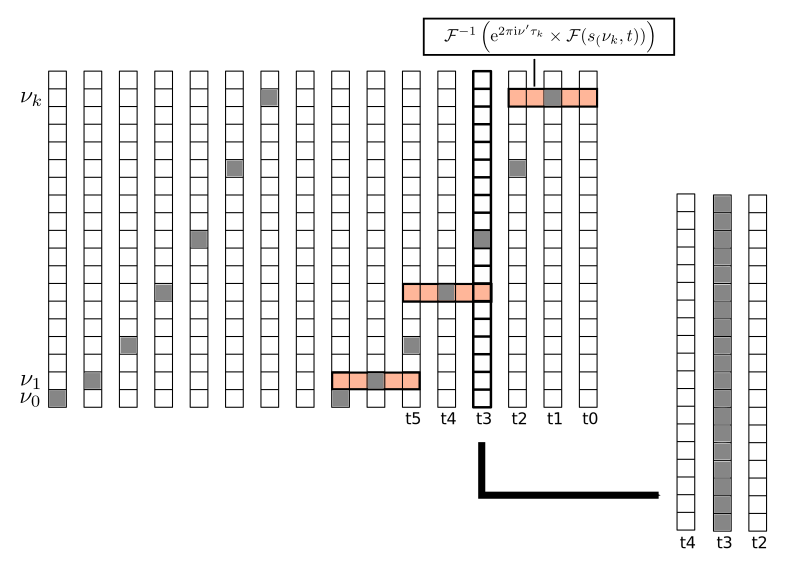
\includegraphics[width=0.9\columnwidth]{cobalt-dedispersion.pdf}
\end{center}
\caption{Coherent dedispersion in \cobalt.}
\label{fig:coherent-dedispersion}
\end{figure}

The approach for \cobalt will therefore be slightly different. In
\cobalt, the data are at a frequency resolution of a few thousand
micro-channels by the time dedispersion is to be performed.  For
\cobalt, $\nu_\mathrm{c}$ will be the central frequency of the output
channel that is closest in frequency to $\nu_k$ to ensure that the
pulse is still dispersed from channel to channel and sub band to sub
band.  Figure~\ref{fig:coherent-dedispersion} illustrates the
situation for all the micro channels that together make up one output
channel. It shows consecutive complex spectra at $t_0$, $t_1$, $t_2$,
$t_3$, $t_4$, $t_5$, etc, at intervals
\begin{equation}
\Delta t = \frac{n_\mathrm{ch}}{\Delta \nu},
\end{equation}
where $n_\mathrm{ch}$ is the number of micro-channels in each time slice and
$\Delta\nu$ is the band width of a sub band. The grey squares indicate
high amplitudes due to a dispersed pulse in the data.

For every micro-channel $k$, one can calculate the delay $\tau_k$ from
Eq.~(\ref{eq:channel-dispersion-delay}), where a negative delay
indicates the pulse arrives at micro-channel $k$ \emph{before} it arrives at
$\nu_\mathrm{c}$. This delay can subsequently be divided into an
integer number of time slices
\begin{equation}
\tau_{k, \mathrm{int}} = \left \lfloor \frac{\tau_k}{\Delta t} + \frac{1}{2}
\right \rfloor,
\end{equation}
and a fraction of a time slice
\begin{equation}
\tau_{k, \mathrm{frac}} = \frac{\tau_k}{\Delta t} - \tau_{k, \mathrm{int}}.
\end{equation}
Note that $|\tau_{k, \mathrm{frac}}| \le \frac{1}{2}$.

In Fig.~\ref{fig:coherent-dedispersion}, time slice $t_3$ is being
dedispersed. The shifted output value for channel $k$ at time $t_i$ is
computed by taking the three-point \fftwforward Fourier transform of
channel $k$ of time slices ${i+\tau_{k, \mathrm{int}}-1}$ until
${i+\tau_{k, \mathrm{int}}+1}$, applying a constant fractional delay
factor in the Fourier domain to compensate for $\tau_{k,
  \mathrm{frac}}$, and taking a three-point \fftwbackward transform
back. The central pixel of the result is the output of channel $k$ at
time slice $i$.

Because these are only three-point Fourier transforms, and we only
need one output value, we can write out the expression
analytically. We first define $t_{-1}$, $t_0$, and $t_{+1}$
to be the complex samples in channel $k$ one time slot before, exactly
at, and one time slot after the time slot $\tau_{k, \mathrm{int}}$
away from the time slot we are currently de-dispersing. Fourier
transforming to the frequency domain, we get
\begin{eqnarray}
f_{-1} & = & \frac{1}{3} \left(t_{-1}\mathrm{e}^{-2\pi\mathrm{i}/3} + t_{0} + t_{+1}\mathrm{e}^{+2\pi\mathrm{i}/3}\right)\\
f_{0}  & = & \frac{1}{3} \left(t_{-1} + t_{0} + t_{+1}\right)\\
f_{+1} & = & \frac{1}{3} \left(t_{-1}\mathrm{e}^{+2\pi\mathrm{i}/3} + t_{0} + t_{+1}\mathrm{e}^{-2\pi\mathrm{i}/3}\right),
\end{eqnarray}
where $\frac{1}{3}$ is the normalization of the Fourier
transform. Multiplying with the phase factor to do the sub-sample
shift gives:
\begin{eqnarray}
f'_{-1} & = & f_{-1} \mathrm{e}^{-2\pi\mathrm{i}\tau_{k, \mathrm{frac}}/3}\\
f'_{0}  & = & f_{0}\\
f'_{+1} & = & f_{+1} \mathrm{e}^{+2\pi\mathrm{i}\tau_{k, \mathrm{frac}}/3}
\end{eqnarray}
The corrected value $t'_0$ is now simply
\begin{equation}
t'_0  =  f'_{-1} + f'_{0} + f'_{+1}.
\end{equation}
There is no need to compute $t'_{-1}$ and $t'_{+1}$, because we do not
need them for this step.

After completing this procedure for time slice $i$, we repeat the
entire process for time slice $i+1$. Because the assumed $\dm$ is
constant during the entire processing stage, $\tau_{k, \mathrm{int}}$
and $\tau_{k, \mathrm{frac}}$ can be computed in advance.

We do still need to evaluate how the change of $\nu_\mathrm{c}$
between blocks of micro-channels affects the transform back to the
time domain, followed by the PPF$+$FFT to the final frequency
resolution. 


%
% Fly's eye mode
%
%
% \section{Fly's eye mode}
% \label{sec:flys-eye}


%
% Final channel separation
%

\section{Final channel separation}
\label{sec:final-channel-separation}

\begin{itemize}
\item Same as \bgp, except at the end of the pipeline, instead of at the
beginning.
\item 16-tap PPF plus FFT in forward direction.
\end{itemize}


%
% Stokes parameters
%
%
% \section{Stokes parameters}
% \label{sec:stokes-parameters}




%
% Bit reduction
%
\section{Bit reduction}
\label{sec:bit-reduction}

\begin{itemize}
\item Scaling and offset re-computed from data every $N$ samples,
  where $N$ is a ``reasonably large'' number.
\item Needs file format definition to agree on where and how to store
  the scales and offsets.
\end{itemize}



\addcontentsline{toc}{section}{References}
\bibliographystyle{aa}
\bibliography{cobalt}


\printindex

\end{document}
